\documentclass{beamer}
\usepackage{subfigure}
\usepackage{graphicx}
\usepackage{caption}
\usetheme{Antibes}
%maths package
\usepackage{amsmath}
\usepackage{xfrac}
\usepackage{nicefrac}

% for numbered equation
\usepackage[utf8]{inputenc}

\title{\textbf{Solution For School Geometry Problems}}
\author{Yogesh Choudhary}


\begin{document}
	\frame{
			\titlepage
		  }
	  
	 \frame{
	  		\frametitle{Question}
	  		\begin{enumerate}
	  		\item 
	  		\textbf{ Two sides AB and BC and median AM of one triangle ABC are respectively equal to sides PQ and QR and median PN of $\Delta$ PQR.Show that:}
	  				
	  			\begin{enumerate}
	  				\item$\Delta$ ABM $\cong$ $\Delta$ PQN  
	  				\item$\Delta$ ABC $\cong$ $\Delta$ PQR
	  			\end{enumerate}
	  	   \end{enumerate}	
  	      }	
	  	
	  	
	    \begin{frame}    	
			\frametitle{Figures}
	    		 Let assume we have two triangles as follows$\to$\\
	    		 
	    	\begin{figure}[!htb]
	    		\begin{minipage}{0.48\textwidth}
	    			\centering
	    			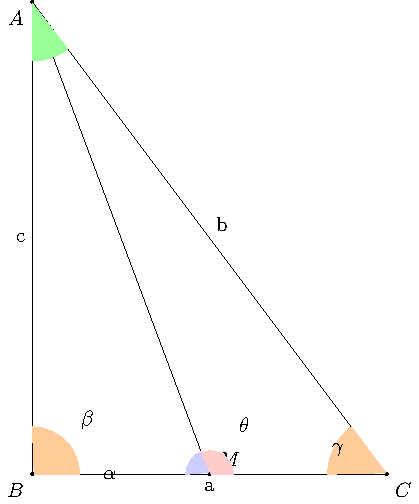
\includegraphics[width=1.5in]{./figures/congurentpicabc.pdf}
	    			\caption{a}
	    			\label{fig:triangle}
	    		\end{minipage}
	    		\hfill
	    		\begin{minipage}{0.48\textwidth}
	    			\centering
	    			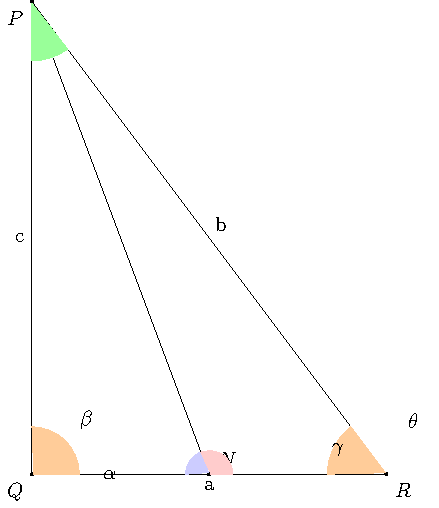
\includegraphics[width=1.5in]{./figures/congurentpicabc2.pdf}
	    			\caption{b}
	    			\label{fig:triangle2}
	    		\end{minipage}	
	    	\end{figure}
	    \end{frame}   
        
        
        \begin{frame}
        	\frametitle{Ans.1}
        	given that $\to$\\
        	
        	\begin{align}
        		AB = PQ\\
        		AM = PN\\
        		BC = QR	
        	\end{align}
        	
        	from equation $\left(3\right)$...
        	
        	\begin{align}
        		\frac{BC}{2} = \frac{QR}{2} \\
        		BM = QN
        	\end{align}
       	\end{frame}
       
       \begin{frame}
       		from fig $\left[1\right]$ and $\left[2\right]$ ...
       	
       		\begin{align}
       			AB = PQ\\
       			AM = PN\\
       			BM = QN\\
       			\implies  \Delta ABM \cong \Delta PQN
       		\end{align}
       \end{frame}
       	
       	\begin{frame}
       		\frametitle{Ans.2}
       		given that $\to$\\
       		\begin{align}
       			AM = PN
       		\end{align}
       		
       		from equation $\left(3\right)$...
       		
       		\begin{align}
       			\frac{BC}{2} = \frac{QR}{2} \\
       			MC = NR
       		\end{align}	
       	\end{frame}
       
     \begin{frame}
     		from equation $\left(9\right)$...
     	\begin{align}
     		\Delta ABM \cong \Delta PQN 
     		\\
     		\implies \angle AMB = \angle PNQ
     		\\
     		180 - \angle AMB = 180 -  \angle PNQ
     		\\
     		\angle AMC = \angle PNR
     	\end{align}
     	
     	from equation $\left(10\right)$,$\left(12\right)$ and $\left(16\right)$...
     	\begin{align}
     		AM = PN
     		\\
     		MC = NR
     		\\
     		\angle AMC = \angle PNR
     		\\
     		\implies  \Delta AMC \cong \Delta PNR
     		\\
     		\implies AC = PR
     	\end{align}
     \end{frame}
 
 	\begin{frame}
 		from equation $\left(1\right)$,$\left(3\right)$ and $\left(21\right)$...
 	
 		\begin{align}
 			AB = PQ\\
 			BC = QR\\
 			AC = QR\\
 			\implies  \Delta ABC \cong \Delta PQR
 		\end{align}
 	\end{frame}
\end{document}